\label{sec:fusion}

본 장에서는 제안하는 퓨전 연산자 \texttt{SNN\_CONV\_POOL\_LIF}의 설계를
기술한다. 먼저 LIF 뉴런의 연산 시맨틱과 표준 TFLM+CMSIS-NN 경로가 본
SNN에서 성능을 잃는 구조적 원인을 분석한 뒤, 이를 해소하는 세 구성 요소
--- Conv+AvgPool 대수적 퓨전, SMLALD 기반 s16$\times$s16 커널, LIF SIMD
에필로그 --- 와 TFLite Micro(TFLM) 커스텀 연산자 통합을 차례로 설명한다.

\subsection{LIF 시맨틱과 표준 커널 경로의 한계}

LIF 뉴런의 이산 시간 동역학은 II장
식~(\ref{eq:lif-bg})--(\ref{eq:lif-reset})와 같다. 막전위 $U$는
타임스텝마다 $\beta$로 감쇠하며 시냅스 입력 $I[t]$를 누적하고, 임계값
$\theta$에 도달하면 스파이크를 발화한 뒤 막전위에서 $\theta$를 감산한다
(감산 리셋). 본 구현은 학습에 사용한 snnTorch Leaky
뉴런\cite{eshraghian2023training}의 시맨틱을 그대로 따르며, 발화한
스파이크가 다음 타임스텝에 출력되는 reset delay 시맨틱을 포함한다. 모든
활성값$\cdot$막전위$\cdot$LIF 파라미터는 Q15 int16이다($\beta=0.9$는
$29{,}491/32{,}768$).

이 모델을 표준 TinyML 스택으로 실행하면 세 가지 갭이 드러난다.

첫째, \textbf{LIF 연산자의 부재}이다. TFLM 빌트인 연산자에는 타임스텝
사이에 상태(막전위, 직전 스파이크)를 유지하는 뉴런 연산이 없으므로,
LIF는 어떤 구성에서도 커스텀 연산자로 구현해야 한다.

둘째, \textbf{CMSIS-NN s16 DSP fast 경로의 커버리지 제약}이다.
CMSIS-NN\cite{lai2018cmsisnn}의 int16 활성$\times$int8 가중치
합성곱에서 DSP 가속 경로(\texttt{arm\_convolve\_fast\_s16})는 im2col
열 길이($k_h \times k_w \times C_{in}$)가 512 미만일 때만 적용된다. 이
한계는 int16$\times$int8 곱(최대 $2^{22}$)을 int32 누산기에 오버플로
없이 누적할 수 있는 항 수가 $2^{31}/2^{22}=512$라는 데서 온다. conv1은
$5\times5\times3=75$로 조건을 만족하지만, conv2는
$5\times5\times32=800$으로 조건을 위배하여 일반 C 커널로 폴백한다.
다음 장에서 실측으로 보이듯, 이 폴백만으로 표준 경로 전체가 스칼라
구현보다 약 2.1배 느려진다.

셋째, \textbf{퓨전 int16 가중치의 미지원}이다. 아래의 Conv+AvgPool
퓨전은 int8 가중치 4개의 합을 새 가중치로 만들므로 값 범위가
$|w|\le508$이 되어 int8에 담기지 않는다. CMSIS-NN s16 커널군은 int8
가중치 전용이므로 이를 수용할 수 없다.

제안 연산자는 이 세 갭을 커스텀 커널 하나로 동시에 해소한다.

\subsection{Conv+AvgPool 대수적 퓨전}

$5\times5$/패딩 2 합성곱 뒤의 $2\times2$/스트라이드 2 평균 풀링은,
평균 풀링이 선형 연산이라는 점을 이용하여 하나의 $6\times6$/스트라이드
2/패딩 2 합성곱과 스칼라 $1/4$의 곱으로 대수적으로 결합할 수 있다.
퓨전 커널 $w_6$은 III장 식~(\ref{eq:w6})으로 빌드 타임에 생성되며,
$1/4$은 나눗셈으로 수행하지 않고 requantize 배율에 흡수하므로
--- 식~(\ref{eq:mfused}) --- 이 변환은 정수 수준에서 등가이다. 그
검증은 다음 장에서 제시한다.

퓨전의 효과는 세 가지다. (i) 타임스텝당 MAC 수가 conv1은
$2{,}457{,}600$에서 $884{,}736$으로, conv2는 $13{,}107{,}200$에서
$4{,}718{,}592$로 줄어 합성곱 합계 기준 약 2.8배 감소한다. (ii) conv 출력과 풀링 입력에 해당하는 중간 텐서가
사라져, 레이어 사이에는 스파이크 텐서($32\times16\times16$,
$64\times8\times8$)만 남는다. (iii) LIF까지 결합하면 requantize
직후의 출력 타일에 뉴런 갱신을 즉시 적용하므로 conv--pool--LIF 사이의
메모리 왕복이 완전히 제거된다. 또한 비퓨전 경로에서 두 번이던
반올림(시프트 절단, 풀링 반올림)이 requantize 한 번으로 줄어든다.
반면 가중치는 int16으로 방출되어 용량이 int8 대비 2배가 되며(conv1
$6{,}912$B, conv2 $147{,}456$B $\approx147.5$KB), conv2 퓨전 가중치는
RAM에 올리지 않고 Flash 상수로 상주시킨다. 이 용량 증가는 배포 가능
영역 분석 장에서 지배 항으로 다시 다룬다. 그림~\ref{fig:fusion}은 퓨전
전후의 연산 구조를 보인다.

\begin{figure}[htbp]
\centering
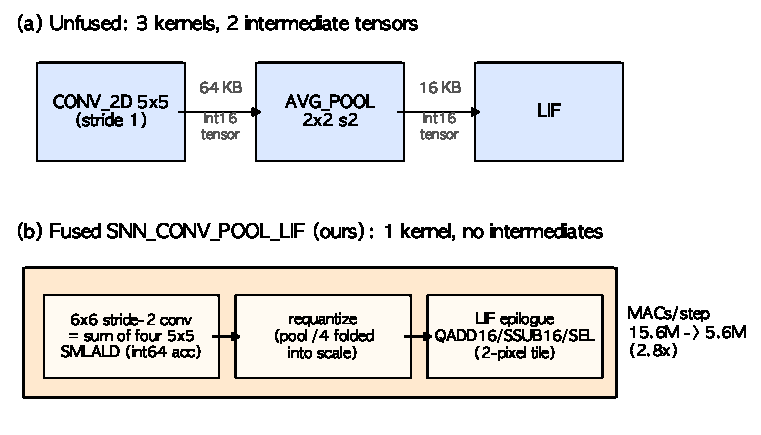
\includegraphics[width=0.9\linewidth]{figures/fig_fusion.pdf}
\caption{제안 퓨전 연산자의 구조. (a) 비퓨전 경로는 커널 3개와 중간
텐서 2개를 거친다. (b) 퓨전 경로는 $6\times6$/스트라이드 2 SMLALD
커널, requantize(풀링 $1/4$을 배율에 흡수), LIF 에필로그가 단일 커널
안에서 이어지며 중간 텐서가 없다(conv 합계 MAC 15.6M
$\rightarrow$ 5.6M/타임스텝).}
\label{fig:fusion}
\end{figure}

\subsection{SMLALD 기반 s16$\times$s16 퓨전 커널}

퓨전 가중치가 int16이므로 s16 활성$\times$s16 가중치 내적을 직접
구현하였다. im2col 구조는 CMSIS-NN
\texttt{arm\_convolve\_fast\_s16}(Apache-2.0)을 준용한다. 입력을
im2col 버퍼에 출력 픽셀 2개(2컬럼) 단위로 전개하고(패딩은 0 채움),
2컬럼이 채워지는 즉시 내적 코어에 전달하며, 홀수 출력 픽셀은 1컬럼
잔여 경로로 처리한다.

내적 코어는 im2col 2컬럼 $\times$ 출력 채널 2개를 동시에 처리하도록
누산기 4개를 유지하고, int16 두 개씩 로드하여 반복당 SMLALD를 4회
실행한다. SMLALD는 듀얼 $16\times16$ 곱을 64비트
누산기에 더하는 Cortex-M7 DSP 명령이다. 64비트 누산은 오버플로 가능성을
제거한다. 곱의 크기는 $|w|\le508<2^{9}$, $|x|\le2^{15}$에서 $2^{24}$
미만인데 conv2의 열 길이가 $6\times6\times32=1{,}152$이므로 최악 누적
합은 int32 범위를 넘지만, int64에서는 실용적인 어떤 열 길이에서도
여유가 있다. 즉 퓨전 커널에는 표준 fast 경로의 512 제약과 같은 커버리지
공백이 없다. 누산이 끝나면 채널별 $(\mathrm{mult},\mathrm{shift})$
파라미터로 \texttt{arm\_nn\_requantize\_s64}를 적용하고
$[-32{,}768,\,32{,}767]$로 클램프한다. \texttt{ARM\_MATH\_DSP}가
정의되지 않은 환경에서는 동일 산술의 스칼라 폴백으로 컴파일되며 결과는
비트 단위로 같다.

\subsection{LIF SIMD 에필로그}

requantize된 2픽셀$\times C_o$ 타일에는 LIF 갱신을 즉시 적용한다.
int16 두 레인을 한 워드에 담아 다음 4단계로 처리한다. (i)
$\beta U \gg 15$: 레인별 $16\times16$ 곱(SMULBB/SMULTB) 후 PKHBT로
재패킹, (ii) QADD16으로 입력을 레인별 포화 가산하여 $\tilde U$ 계산
--- 식~(\ref{eq:lif-bg})의 갱신, (iii) SSUB16으로 $\tilde U-\theta$를
레인별로 계산하면서 APSR.GE 플래그 설정, (iv) SEL로 분기 없이 다음
막전위(발화 레인은 $\tilde U-\theta$, 비발화 레인은 $\tilde U$)와
스파이크 값(발화 $32{,}767$, 비발화 0)을 선택한다. 출력은 직전 스텝의
스파이크를 내보내는 reset delay 시맨틱을 따른다. SIMD 경로는 관련
포인터가 모두 4바이트 정렬일 때만 진입하며, 스칼라 폴백과 비트 단위로
동일하다(전수 검증은 다음 장에서 제시).

\subsection{TFLM 커스텀 연산자 통합과 구현 제약}

제안 커널은 TFLM\cite{david2021tflm}에 커스텀 연산자
\texttt{SNN\_CONV\_POOL\_LIF1/2}와 \texttt{SNN\_LIF\_OUT}으로 등록되고,
마지막 FC 층은 빌트인 \texttt{FULLY\_CONNECTED}(CMSIS-NN int16x8)를
그대로 사용한다(\texttt{MicroMutableOpResolver}$\langle4\rangle$).
활성 텐서의 양자화는 scale $1/32{,}768$(Q15), zero point 0이며 스파이크
값은 전 레이어 $32{,}767$이다. 커널 Prepare 단계에서 채널별 유효 배율
$\mathrm{eff}=s_{in}\,s_{w}[c]/s_{out}$을 \texttt{QuantizeMultiplier}로
$(\mathrm{mult},\mathrm{shift})$에 분해한다.

메모리는 TFLM 아레나로 일원화하였다. 타임스텝을 넘어 유지되어야 하는
LIF 상태(막전위$\cdot$직전 스파이크)와 채널별 mult/shift 테이블은
\texttt{AllocatePersistentBuffer}로, Invoke 동안만 필요한 im2col
버퍼는 \texttt{RequestScratchBufferInArena}로 할당하며, 활성 텐서는
아레나 메모리 플래너가 배치한다. 그 결과 TFLM 경로의 SNN 관련 RAM은
전부 단일 아레나 안에서 관리되고 별도의 정적 배열이 없다. LIF 상태는
이미지 경계에서 재설정한다.

구현 제약은 두 가지다. batch 1 전용이며, 내부 타일이
\texttt{int16\_t tile[2*64]}로 고정되어 있어 출력 채널 수
$C_o \le 64$를 가정한다. 현 모델(32/64채널)은 이를 충족하며, 제약
완화 조건은 배포 가능 영역 분석 장에서 논의한다.
